\documentclass[a4paper]{article}

%% Language and font encodings
\usepackage[english]{babel}
\usepackage[utf8x]{inputenc}
\usepackage[T1]{fontenc}
\usepackage{booktabs}
\usepackage{amsmath}
\usepackage{amsthm}
\usepackage{amsfonts}
\usepackage[colorlinks=true, allcolors=black]{hyperref}
\usepackage{graphicx}
\usepackage[hypcap=false]{caption}
\usepackage{subcaption}
\usepackage{amssymb}
\usepackage{fullpage,graphicx,textcomp,float,gensymb,wrapfig}
\usepackage{natbib}
\usepackage{algorithm}
\usepackage[noend]{algpseudocode}

\setcitestyle{round}

\captionsetup[algorithm]{singlelinecheck=off}

\algnewcommand{\LeftComment}[1]{\Statex \(\triangleright\) #1}

\renewcommand\algorithmicthen{}
\renewcommand\algorithmicdo{}

\title{Case Combinatorische Optimalisatie 2017}
\author{Philip Boeken \and Stein Heijjer \and Koen Meijer}

\begin{document}
\maketitle
\section{Introduction}
In the course Combinatorische Optimalisatie the students are given a case in which they have to create an algorithm for solving a vehicle routing problem with time windows and multiple products, coined 'Verolog'. We have produced an algorithm which divides Verolog into a scheduling problem and a routing problem. For the scheduling problem we created a heuristic from scratch, and for the routing problem we created a heuristic based on the VRP algorithm given by \citeauthor{clarkewright1964} (\citeyear{clarkewright1964}). This report shows a proof of the NP-completeness of the Verolog problem and presents our algorithm along with an analysis of its time complexity. Then experimental running times are analysed, and results and the general design choices are discussed.  

\section{NP-completeness}
Proving that the Verolog problem is NP-complete requires two proofs (Lecture 2, slide 73): 1. That the problem is in NP, 2. That all other problems in NP polynomially transform to our problem.

The book Algorithms by \citeauthor{Dasgupta2006} (\citeyear{Dasgupta2006}) gives the following definition for NP: \\

\emph{We know what a search problem is: its defining characteristic is that any proposed solution can be quickly checked for correctness, in the sense that there is an efficient checking algorithm $C$ that takes as input the given instance $I$ (the data specifying the problem to be solved), as well as the proposed solution S, and outputs true if and only if S really is a solution to instance $I$. Moreover the running time of $C(I,S)$ is bounded by a polynomial in $|I|$, the length of the instance. We denote the class of all search problems by NP.} \\

For assignment 2 we have proposed a validator, which complies with the restrictions of algorithm $C$ specified by Daspgupta. This implies that Verolog is a search problem, and therefore is in NP.

Proving that Verolog is NP-complete requires proving that all problems in NP polynomially reduce to Verolog. Dasgupta's definition of reduction of search problem $A$ to search problem $B$ is the following: \\

\emph{A reduction from search problem $A$ to search problem $B$ is a polynomial-time algorithm $f$ that transforms any instance $I$ of $A$ into an instance $f(I)$ of $B$, together with another polynomial-time algorithm $h$ that maps any solution $S$ of $f(I)$ back into a solution $h(S)$ of $I$. If $f(I)$ has no solution, then neither does $I$.} \\

It is widely known that the Euclidean Travelling Salesman Problem (TSP) is NP-complete \citep{papadimitriou1977}. In Dasgupta's definition of polynomial reduction, let $A$ denote the Euclidean TSP, and let $B$ denote Verolog. Then, $I$, $f(I)$ and $h(S)$ can be defined as the following:
\begin{itemize}
	\item[$I$:] Let $G=(V,E)$ denote the complete graph with cities ($V$) and connections between these cities ($E$). Also, let $w(e_i)$ denote the Euclidean distance between $v_j, v_k \in e_i$ of edge $e_i \in E$.
	\item[$f(I)$:] Choose the following Verolog instance parameters: \textbf{Days} = 2, \textbf{Capacity} = $|V|$,  \textbf{Max trip distance} = $\sum_{i=1}^{|E|}w(e_i)$ (or some other at least as large number), \textbf{Coordinates}: Match every node $v \in V$ with a coordinate, such that the weights $w(e) \quad \forall e \in E$ comply with the Euclidean distance between every two coordinates, \textbf{Depot coordinate}: Pick a coordinate randomly from the assigned coordinates, \textbf{Vehicle cost}: $1$, \textbf{Vehicle day cost}: 1, \textbf{Distance cost}: $1$, \textbf{Tools}: one tool with input values '1 0 $|V|$ 0', \textbf{Requests} = $|V|-1$: Match every coordinate (except the depot) with a request which has to be delivered on day 1, has to be picked up on day 2, and requires one tool of type 1.
	\item[$h(S)$:] Revert the mapping of $V$ to coordinates (as in $f(I)$), which creates a set of vertices $V$. The order in which the requests are delivered in $S$ is the TSP route. 
\end{itemize}
Using these functions, an algorithm for solving Verolog will always find a routing which lets one vehicle handle all deliveries. Since the Verolog algorithm has to minimize the distance of this vehicle, the edges between the request locations will be the same as the edges between the nodes of the Euclidean TSP. Moreover, the Verolog algorithm will not find a solution which visits the depot more than twice (start and end of tour), since the capacity of the vehicle is larger than the total amount of tools needed. Because of this fact and the fact that every delivery is handled once, no node of the solution $h(S)$ will be visited more than once.

\section{The Algorithm}
The Verolog algorithm solves two semi-distinct problems. First, all request are assigned to days within the total timespan of the problem. Such a configuration is called a 'schedule'. Given such a schedule, for each day a set of trips is made. A trip is on its turn defined as an ordered list of requests and depot visits. When a routing is created, it is optimized using 2-opt. In this section, all sub-algorithms are individually explained, and then combined into the main algorithm. Along with the explanation of a sub-algorithm, its time complexity is analysed. At the beginning of the pseudocode of every sub-algorithm, the total time complexity that sub-algorithm is given by the "\textbf{Time complexity:}" statement. Throughout the pseudocode, the most notable contributions of time complexity by individual loops and statements are given. \\

The function which creates a schedule is expected to return a schedule in which all deliveries are planned within the relevant time window, and all pickups are planned on the relevant days. This is done in the class InitSchedule. The schedule is created based on Algorithm \ref{schedule}. The 'minimum' that is used, is defined by the minimum inventory at the beginning of a day over all tools. For every day, the mutations of the inventory are the subtractions of all deliveries, and additions of all pickups. In practice this would be equivalent to the number of tools which do not have to be picked up and delivered on the same trip. Therefore, the minimum provides a theoretical upper bound of the inventory: no algorithm can have a lower tool use than this upper bound. In every iteration, the mutations to the schedule are purely random. When this mutation results in a lower minimum inventory, the mutation is reversed. When the minimum increases, the iterator is set to 0. When the minimum remains the same, the iterator is raised with a value of 1. Therefore, the algorithm only returns a schedule when 1500 consecutive iterations have not improved the theoretical upper bound of the inventory. Maximizing this theoretical upper bound of the inventory provides a forgiving schedule: when creating a routing from this schedule, the restriction on tool use is as weak as possible. \\ Algorithm \ref{schedule} is the only randomized part of the total algorithm. It can be seen that there are $N^{\text{\#request days}}$ possible options for the schedule to be in, where $\#\text{request days}$ is the number of days a request can be delivered on. In practice we cap this iteration by stopping the scheduler when no improvement is seen in 1500 iterations. \\


\begin{algorithm}
	\caption{The algorithm for creating a schedule}
	\label{schedule}
	\begin{algorithmic}
		\State \textbf{Input:} The problem instance
		\State \textbf{Output:} A schedule
		\State \textbf{Time complexity:} Stochastic
		\For{\textbf{each} Request in the instance} \Comment{$\mathcal{O}(N)$}
			\State Add the request to the first day of it's time window 
		\EndFor
		\State Get current minimum
		\While{$i < 1500$} \Comment{Stochastic runtime}
			\State Randomly pick a day on which a delivery is planned
			\State Randomly pick a delivery which is planned on that day
			\State Randomly pick a day within the time window of the delivery, and relocate the delivery to that day
			\State Get new minimum
			\If{New minimum < current minimum}
				\State Undo the delivery change of this iteration
			\Else
				\If{New minimum > current minimum}
					\State $i \gets 0$
				\Else
					\State $i \gets i+1$
				\EndIf
			\EndIf
		\EndWhile
	\end{algorithmic}
\end{algorithm}

When a schedule is created, it must be transformed into a routing. This is done using Algorithm \ref{routing}. Note that this algorithm takes a schedule for a single day as input. Therefore, the main algorithm has to repeat this algorithm for every day. This algorithm is based on the VRP algorithm proposed by \citeauthor{clarkewright1964} (\citeyear{clarkewright1964}). \\
First, an initial routing is created. This is done in such a way that an individual trip is made for every request. Then a savings list is created. This is a list of pairs of requests (deliveries and pickups). For every pair of requests, the saving is calculated: the sum of the distance between the depot and each request, reduced by the distance between both requests. This list is sorted on the saving value, in a descending order. \\
After this savings list is created, the algorithm will start looping through this list. Per iteration the algorithm checks whether the requests of a savings pair are currently contained by different trips. If this is the case, and the maximum distance is not exceeded, both trips are concatenated into a new trip. If the current routing is not yet valid in terms of tool use, only trips will be added that have a benefit to this tool use. This would mean that a trip would do a pickup before a delivery, so the tools needed from the depot will be lower. Once the routing is valid in terms of tool use, all valid savings pairs will be added. It can be seen in Algorithm \ref{routing} that our implementation of Clarke Wright itself has a runtime of $\mathcal{O}(N^2)$. However, since Clarke Wright is still part of the loop in search of a valid routing, this algorithm can in theory be run an infinite number of times. \\


\begin{algorithm}
	\caption{The algorithm for creating a routing}
	\label{routing}
	\begin{algorithmic}
		\State \textbf{Input:} A schedule for one day
		\State \textbf{Output:} A routing
		\State \textbf{Time complexity:} $\mathcal{O}(N^2)$
		\State Add a trip for each request 
		\State Create a savings list \Comment{$\mathcal{O}(N^2)$}
		\For{\textbf{each} Pair of requests in the savings list} \Comment{$\mathcal{O}(N)$}
			\State Get the trips that contain the requests
			\If{The trips are not the same}
				\State Concatenate the trips into a new trip \Comment{$\mathcal{O}(N)$}
				\If{The new trip is valid}
					\State Check benefit
					\State Check validChange
					\If {Benefit and validChange}
						\State Delete old trips
						\State Add new trip
					\EndIf
				\EndIf
			\EndIf
		\EndFor
	\end{algorithmic}
\end{algorithm}

Given a day of routing, the algorithm tries to decrease the costs by first using 2-opt, and secondly by merging trips. The 2-opt algorithm first creates a savings list. This list is created for a single trip: for each pair of requests in the trip the current costs of the trip are calculated, and the costs of the trip when the order of the handling of the relevant requests is reversed are calculated. When swapping these requests provides lower costs, the pair of requests are stored in the savings list, along with its relevant saving. When the savings of all pairs of requests are calculated, this list is sorted on the saving value, in a descending order. Then, these savings are executed. However, every time a saving is executed (i.e. two requests are swapped) the savings list is recalculated. Eventually, when no savings are possible, the 2-opt algorithm halts. \\ Then the optimization algorithm merges trips when possible. The possibility of merging trips is determined by whether the merged trip exceeds the maximum trip distance or not. 

The 2-opt has a runtime of $\mathcal{O}(N^3)$. In every iteration of the 2-opt a trip is considered. For this trip a savings list is created. If this list yields an improvement, the list is created again. Therefore this list gets created at most N times. Since creating the savings list is $\mathcal{O}(N^2)$, the whole 2-opt algorithm takes $\mathcal{O}(N^3)$. \\

\begin{algorithm}
	\caption{The algorithm for optimizing a routing}
	\label{2opt}
	\begin{algorithmic}
		\State \textbf{Input:} A routing
		\State \textbf{Output:} A (optimized) routing
		\State \textbf{Time complexity:} $\mathcal{O}(N^3)$
		\For{\textbf{each} Day in the routing} \Comment{$\mathcal{O}(N)$}
			\For{\textbf{each} Trip on this day of the routing}
				\State Ready $\gets$ false
				\While{Not ready}
					\State Create a savings list \Comment{$\mathcal{O}(N^2)$}
					\For{\textbf{each} Pair of requests in the savings list}
						\State Swap requests
						\If{The new trip is valid}
							\State Ready $\gets$ false
							\State Break
						\Else
							\State Undo swapping
							\State Ready $\gets$ True
						\EndIf
					\EndFor
				\EndWhile
			\EndFor
			\State Merge trips \Comment{$\mathcal{O}(N)$}
		\EndFor
	\end{algorithmic}
\end{algorithm}

The main algorithm is depicted in Algorithm \ref{main}. All in all this algorithm has a stochastic runtime due to the randomized parts of the algorithm. However, in practice we only see the random elements needed in the first test instance. Even in this case the random elements are not repeated more than 4 or 5 times. Which would bring the total runtime to around 30 seconds. \\

\begin{algorithm}
	\caption{The main algorithm}
	\label{main}
	\begin{algorithmic}
		\State \textbf{Input:} A problem instance
		\State \textbf{Output:} A routing
		\State \textbf{Time complexity:} Stochastic
		\While{The routing is not valid}
			\State Create a schedule using Algorithm \ref{schedule} \Comment{Stochastic time}
			\For{\textbf{each} Day in the schedule} \Comment{$\mathcal{O}(N)$}
				\State Create a routing using Algorithm \ref{routing} \Comment{$\mathcal{O}(N^2)$}
			\EndFor
		\EndWhile
		\State Improve the routing using Algorithm \ref{2opt} \Comment{$\mathcal{O}(N^3)$}
	\end{algorithmic}
\end{algorithm}

We chose this design because we valued validity of our algorithm over optimality. Therefore we decided to only optimize the theoretical upper bound of the inventory in the scheduler. This is done to make the schedule as easy to make valid as possible. Furthermore we chose Clarke Wright because we wanted an algorithm that could find a good initial solution, without a long runtime. We always had in mind that we needed to do an optimization heuristic at some point, which in our case became 2-opt. But since 2-opt would work faster on a good initial solution, we decided to use Clarke Wright as it finds this solution relatively quickly.

\section{Results}
For our experimental runtime analysis we used ORTEC\_Test\_01, this is because this is the “hardest” instance to find a valid solution for in terms of tool use. This is the only instance where our algorithm needs to do more than one iteration of the scheduler to find a valid routing. In the table below the average runtime for different parts of the algorithm is shown. As can be seen in Table \ref{results}, the algorithm doesn’t always find a valid routing on the first try. On average it takes the algorithm 9,1 seconds to find a valid routing. After this 2-opt still has to be done, which brings the total runtime to 15,7 seconds. Figure \ref{fig:results} shows a box plot of the runtime to find a valid solution. It can be seen that the median remains relatively low at 5,7 seconds.  The upper quartile also stays relatively low. But as with all random algorithms big outliers can be found, which can here be seen at around 25 seconds. This outlier means 5 tries before the scheduler found a valid solution.

\begin{table}
	\centering
	\caption{Numerical results}
	\label{results}
	\begin{tabular}{ccccc}
		\toprule
		Initial Schedule & Clarke Wright & Initial Routing & Valid Routing & 2-opt \\ \midrule
		1.9 seconds & 3.2 seconds & 5.1 seconds & 9.1 seconds & 6.6 seconds \\
		\bottomrule
	\end{tabular}
\end{table}

\begin{figure}
	\center
	\caption{Runtime in seconds}
	\label{fig:results}
	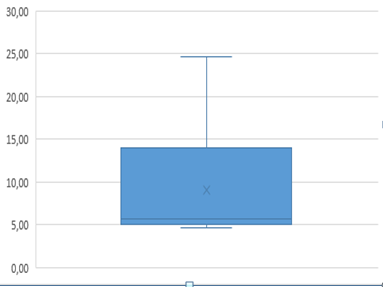
\includegraphics[width=.5\textwidth]{results.PNG}
\end{figure}

Our algorithm does not use any approximations, therefore it could in theory perform relatively bad. The lower bound of our algorithm is a separate route for every request, in the case no savings are possible. This could be used for an approximation, however the schedule still remains variable. Since this is determined by a randomiser we cannot give any guaranteed value our algorithm will find. \\
 
As mentioned before, our algorithm favours validity over optimality. This is why we decided to use the randomiser in the schedule maker. Clarke Wright also aggressively tries to make a routing valid first, before implementing all possible savings. In practice some instances are easy to make valid, in this case our algorithm performs worse than is probably necessary. If we would’ve had more time we would implement a system that checks how hard an instance is to solve. In that case our scheduler could be more cost minded, as well as Clarke Wright. This is also why we decided to use 2-opt at the end of the algorithm. Since 2-opt only looks at cost, we decided it would be good to run it over our already valid solution, to make it more cost optimal. \\

In terms of runtime we could still improve the schedule maker. Since this is currently a random algorithm it is not very time efficient. We could use another algorithm, that tries to maximize the minimum tools needed in a schedule. This algorithm would probably be faster than our randomiser. The randomiser does however have the advantage that multiple options are explored in case a schedule can’t be made valid by Clarke Wright, and therefore has the added benefit of variance in the schedule.


\bibliographystyle{plainnat}
\bibliography{references}


\end{document}
